\section{Optimale løsning}
\label{sec:eksistens}
Hvis løsnings mængden til et lineært programmerings problem ikke er tom, må der være en løsning til problemet.
Men bare fordi der eksistere en løsning, behøver der ikke eksistere en optimal løsning. 
%\begin{defn}
%Lad $P=\{\vec{x} \in \mathds{R}^n| A \vec{x} \geq b, \vec{x} \geq \vec{0}\} \neq \emptyset$ være en polyide, svarende til bibetingelserne til det lineære minimerings problem $\vec{c}^T\vec{x}$.
%Da siges en vektor $\vec{x^*}\in P$ at være \textbf{optimal}, hvis $\vec{c}^T\vec{x^*}\leq \vec{c}^T\vec{x}$ for alle $\vec{x}\in P$
%\end{defn}
Betragt tilfældet, hvor der eksistere en vektor i løsningsmængden, hvor det er muligt at lægge en vilkårlig stor vektor til, og summen stadig er indholdt i løsnings mængden.
Er det tilfældet siges løsningsmængden at indeholde en linje.
\begin{defn}[Linje]
Lad $P\subseteq \mathds{R}^n $ være en polyide, da indeholder $P$ en \textbf{linje}, hvis $\vec{x}+\lambda\vec{d} \in P$ for alle $\lambda \in \mathds{R}^n$, hvor $\vec{x}\in P$ og $\vec{d} \in \mathds{R}^n$.
\end{defn}
Hvis løsningsmængden indholder en linje, så må objektfunktion nødvendigvis kunne tage en vilkårlig stor værdi, og løsningen vil være lig $-\infty$ i tilfældet af, at objektfunktionen skal minimeres. 
Det antyder derfor, at objektfunktionen skal være begrænset, for at der eksistere en optimal løsning.
\begin{defn} [Begrænset]
Lad $S \subset \mathds{R}^n$, da er $S$ begrænset, hvis der eksistere en konstant $K$ så $\forall \vec{x} \in S: \langle \vec{x}, \vec{x} \rangle \leq K$
\end{defn}
Det viser sig, at hvis løsnings mængden ikke er tom og ikke indeholder en linje, så er der en optimal løsning, som vil være en mulig basisløsning, det vil sige, at løsningen findes i et skærings punkt af $n$ lineært uafhængige bibetingelser.
\begin{stn}[Eksistens af optimal løsning]
Lad $P=\{\vec{x} \in \mathds{R}^n| A \vec{x} \geq b \} \neq \emptyset$ være en polyide, svarende til bibetingelserne til det lineære minimerings problem $\vec{c}^T\vec{x}$. Hvis $P$ ikke indeholder en linje, da vil der eksistere en optimal løsning $\vec{x^{**}}$ som er en mulig basisløsning.
\label{stn:eksistens}
\end{stn}
Sætningen bevises med et medføre bevis, ved at finde en vektor $\vec{x}$ i løsningsmængden også konstruere en mulig basisløsning ud fra vektoren. 
Ved at finde en retnings vektor $\vec{d}$, som minimere objektfunktionen, og så lægge et multiplum af $\vec{d}$ til $\vec{x}$ indtil, at summen gør en ny bibetingelse aktiv. 
Det vil altid være muligt at finde sådan en bibetingelse, da løsningsmængden ikke indeholder en linje.
Processen gentages til, vektoren har $n$ lineært uafhængige aktive bibetingelser, se Figur \ref{fig:eksistens}.
\begin{figure}
\begin{center}
	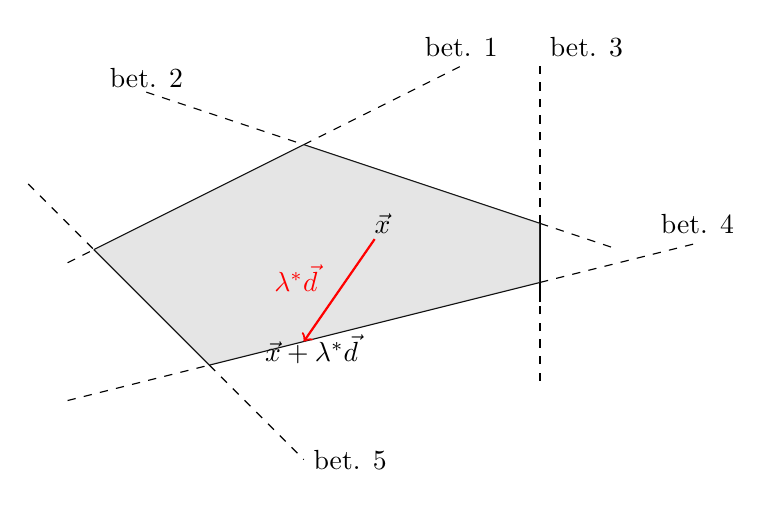
\begin{tikzpicture}[ latex
  s/.style={width=0}]

  %ligning 1
	\draw[domain=-1:-2/3,variable=\x,dashed] 	plot({\x},{0.5*\x+1});
	\draw[domain=-2/3:2,variable=\x] 			plot({\x},{0.5*\x+1});
	\draw[domain=2:4,variable=\x,dashed] 	plot({\x},{0.5*\x+1}) node[above] {bet. 1};
	
  %ligning 2
  	\draw[domain=0:2,variable=\x,dashed] 	plot({\x},{-(1/3)*\x+8/3}) node[above] at (0,2.6) {bet. 2} ;
	\draw[domain=2:5,variable=\x] 			plot({\x},{-(1/3)*\x+8/3});
	\draw[domain=5:6,variable=\x,dashed] 	plot({\x},{-(1/3)*\x+8/3});
	

  %ligning 3
  	\draw[domain=-1:0,variable=\y,dashed] 	plot({5},{\y});
	\draw[domain=0:1,variable=\y] 			plot({5},{\y});
	\draw[domain=1:3,variable=\y,dashed] 	plot({5},{\y}) node[above right] {bet. 3};
	
  %ligning 4
	\draw[domain=-1:4/5,variable=\x,dashed] 	plot({\x},{0.25*\x-1});
	\draw[domain=4/5:5,variable=\x] 			plot({\x},{0.25*\x-1});
	\draw[domain=5:7,variable=\x,dashed] 	plot({\x},{0.25*\x-1}) node[above] {bet. 4};
	
  %ligning 5
  	\draw[domain=-1.5:-2/3,variable=\x,dashed] 	plot({\x},{-\x}) ;
	\draw[domain=-2/3:4/5,variable=\x] 			plot({\x},{-\x});
	\draw[domain=4/5:2,variable=\x,dashed] 	plot({\x},{-\x}) node[right] {bet. 5} ;

  %løsningsmængden skraveret
	\fill[gray!80,nearly transparent] (4/5,-4/5) -- (-2/3,2/3) -- (2,2) -- (5,1) --(5,0.25) --  cycle;
	
  % vektor x
	\node[] (x) at (3,1) {$\vec{x}$};
	\draw[thick, color=red, ->](2.9,0.8) -- (2,-0.5) node[above, yshift=0.5 cm, xshift=-0.1 cm] {$\lambda^* \vec{d}$} ;
	\node[] (x) at (2.1, -0.6) {$\vec{x}+\lambda^* \vec{d}$};
 
\end{tikzpicture}
	\captionof{figure}{Der ligges et multiplum af en retnings vektor til vektor $\vec{x}$ til at summen gør betingelse $4$ aktiv.}
	\label{fig:eksistens}
\end{center}
\end{figure}
Da objektfunktionen til enhver vektor i løsningsmængden, derfor er mindre eller lig objektfunktionen til en mulig basisløsning, må den optimale løsning, være en mulig basisløsning.
\begin{proof}
Da $P$ ikke er tom må der eksistere en vektor $\vec{x} \in P$.
Antag at $\vec{x}$ ikke er en mulig basisløsning, da vil $I = \{i | \vec{a_i}^T\vec{x} = b_i\}$, hvor $\vec{a_i}^T\vec{x}=b_i$ er aktive lineære uafhængige bibetingelser, indeholde færre end $n$ elementer. 
Nu konstrueres en mulig basisløsning $\vec{x^*}$, med udgangspunkt i $\vec{x}$ så $\vec{c}^T\vec{x^*}\leq \vec{c}^T\vec{x}$.
Da $|I|<n $ må $span(\{a_i | i \in I\})$ være et ægte underrum til $\mathds{R}^n$, hvorfor der eksistere en vektor $\vec{d} \in \mathds{R}^n$ så $\vec{a_I}^T\vec{d}=0$ for alle $i \in I$. 
Vælg nu fortegn på $\vec{d}$ så $\vec{c}^T\vec{d} \leq 0$, da vil $\vec{c}^T(\vec{x}+\lambda\vec{d}) \leq \vec{c}^T\vec{x}$ hvor $\lambda$ er en positiv skalar.
Da $P$ er begrænset, og derfor ikke indeholder en linje, må der være et $\lambda'$ som gør, at $\vec{x}+\lambda'\vec{d} \notin P$, hvorfor at der for et $\lambda^*$ må gælde, at $\vec{a_j}^T(\vec{x}+\lambda^* \vec{d}) = b_j$, for $j \notin I$.
Bemærk at $\vec{x}+\lambda^*\vec{d} \in P$, da $\vec{a_i}^T(\vec{x}+\lambda\vec{d})= \vec{a_i}^T\vec{x} = b_i$, for $i \in I$, hvorfor alle aktive bibetingelser stadig er overholdt.
Antag nu at $\vec{d}$ er lineært afhængig af andre bibetingelser end $\vec{a_j}$, da vil $\vec{a_j}$ også være lineært afhæng af dem, hvorfor det følger af Sætning \ref{stn:PQ}, at man kan se bort fra dem, og $\vec{x}+\lambda \vec{d} \in P$ må derfor stadig gøre sig gældende. 
Da $\vec{d}$ er lineært afhængig af $\vec{a_j}$, må det medfører, at da $\vec{d}$ er lineært uafhængig af $\vec{a_i}$ så må $\vec{a_j}$ også være det. 
Derfor kan $j$ tilføjes til $I$. 
Gentag til at $I$ indeholder $n$ lineært uafhængige vektorer, hvorefter det følger af Definition \ref{def:basislosning} at en basisløsning er konstrueret, og da løsningen er konstrueret ud fra en mulig løsning uden at overtræde nogle betingelser, må det være en mulig basisløsning.\\
Da $\vec{x^*}$ er konstrueret ud fra en vilkårlig vektor $\vec{x}\in P$ medføre det, at en mulig basisløsning altid vil opfylde $\vec{c}^T\vec{x^*} \leq \vec{c}\vec{x}$ for en hver ikke mulig basisløsning. 
Da der kun er en endelig mængde mulige basisløsninger, må der være en vektor $\vec{x^{**}}$, som opfylder, at $\vec{c}^T\vec{x^{**}}\leq \vec{c}^T\vec{x^*}$ for alle andre mulige basisløsninger, hvorfor at $\vec{x^{**}}$ er en optimal løsning.
\end{proof}
Sætning \ref{stn:eksistens} kan omskrives en smugle, så i stedet for at kravet er, at løsningsmængden ikke har en linje, så er det at objekt funktionen til løsningsmængden er begrænset.
\begin{kor}
Lad $f(\vec{x}) = \vec{c}^T\vec{x}$ betegne et lineært minimerings programmerings problem, med mulige løsningsmængde $\mathcal{F} \neq \emptyset$. 
Da eksistere en optimal løsning, som er en mulig basisløsning, hvis der eksistere et $K \in \mathds{R}$ så $|f(\mathcal{F})| \leq K$ 
\label{kor:eksistens}
\end{kor}
Korollar \ref{kor:eksistens} bevises ved et medføre bevis.
\begin{proof}
Lad  $K \in \mathds{R}$ så $|f(\mathcal{F})| \leq K$, da må der for et hvert $\vec{x} \in P$ og $\vec{d} \in \mathds{R}^n$ eksistere et $\lambda$ så $f(\vec{x}+\lambda \vec{d}) = K$, og da $f$ er lineær, følger det, at $\mathcal{F}$ ikke kan indeholde en linje. 
Da $\mathcal{F} \neq \emptyset$ følger det af Sætning \ref{stn:eksistens}, at er eksistere en optimal løsning, som er en mulig basisløsning til det lineære minimerings programmerings problem.
\end{proof}
Det betyder, at hvis der til et lineært programmerings problem skal eksistere en optimal løsning, så må løsningsmængden ikke indeholde en linje og objektfunktion på løsningsmængden skal være begrænset. 
Er det ikke tilfældet må objektfunktionen kunne tage værdierne $\infty$ og $-\infty$, og det vil derfor være løsningen på problemet, alt afhængig af om, der er tale om et henholdsvis maksimering eller minimerings problem.

